\documentclass[1p]{elsarticle_modified}
%\bibliographystyle{elsarticle-num}

%\usepackage[colorlinks]{hyperref}
%\usepackage{abbrmath_seonhwa} %\Abb, \Ascr, \Acal ,\Abf, \Afrak
\usepackage{amsfonts}
\usepackage{amssymb}
\usepackage{amsmath}
\usepackage{amsthm}
\usepackage{scalefnt}
\usepackage{amsbsy}
\usepackage{kotex}
\usepackage{caption}
\usepackage{subfig}
\usepackage{color}
\usepackage{graphicx}
\usepackage{xcolor} %% white, black, red, green, blue, cyan, magenta, yellow
\usepackage{float}
\usepackage{setspace}
\usepackage{hyperref}

\usepackage{tikz}
\usetikzlibrary{arrows}

\usepackage{multirow}
\usepackage{array} % fixed length table
\usepackage{hhline}

%%%%%%%%%%%%%%%%%%%%%
\makeatletter
\renewcommand*\env@matrix[1][\arraystretch]{%
	\edef\arraystretch{#1}%
	\hskip -\arraycolsep
	\let\@ifnextchar\new@ifnextchar
	\array{*\c@MaxMatrixCols c}}
\makeatother %https://tex.stackexchange.com/questions/14071/how-can-i-increase-the-line-spacing-in-a-matrix
%%%%%%%%%%%%%%%

\usepackage[normalem]{ulem}

\newcommand{\msout}[1]{\ifmmode\text{\sout{\ensuremath{#1}}}\else\sout{#1}\fi}
%SOURCE: \msout is \stkout macro in https://tex.stackexchange.com/questions/20609/strikeout-in-math-mode

\newcommand{\cancel}[1]{
	\ifmmode
	{\color{red}\msout{#1}}
	\else
	{\color{red}\sout{#1}}
	\fi
}

\newcommand{\add}[1]{
	{\color{blue}\uwave{#1}}
}

\newcommand{\replace}[2]{
	\ifmmode
	{\color{red}\msout{#1}}{\color{blue}\uwave{#2}}
	\else
	{\color{red}\sout{#1}}{\color{blue}\uwave{#2}}
	\fi
}

\newcommand{\Sol}{\mathcal{S}} %segment
\newcommand{\D}{D} %diagram
\newcommand{\A}{\mathcal{A}} %arc


%%%%%%%%%%%%%%%%%%%%%%%%%%%%%5 test

\def\sl{\operatorname{\textup{SL}}(2,\Cbb)}
\def\psl{\operatorname{\textup{PSL}}(2,\Cbb)}
\def\quan{\mkern 1mu \triangleright \mkern 1mu}

\theoremstyle{definition}
\newtheorem{thm}{Theorem}[section]
\newtheorem{prop}[thm]{Proposition}
\newtheorem{lem}[thm]{Lemma}
\newtheorem{ques}[thm]{Question}
\newtheorem{cor}[thm]{Corollary}
\newtheorem{defn}[thm]{Definition}
\newtheorem{exam}[thm]{Example}
\newtheorem{rmk}[thm]{Remark}
\newtheorem{alg}[thm]{Algorithm}

\newcommand{\I}{\sqrt{-1}}
\begin{document}

%\begin{frontmatter}
%
%\title{Boundary parabolic representations of knots up to 8 crossings}
%
%%% Group authors per affiliation:
%\author{Yunhi Cho} 
%\address{Department of Mathematics, University of Seoul, Seoul, Korea}
%\ead{yhcho@uos.ac.kr}
%
%
%\author{Seonhwa Kim} %\fnref{s_kim}}
%\address{Center for Geometry and Physics, Institute for Basic Science, Pohang, 37673, Korea}
%\ead{ryeona17@ibs.re.kr}
%
%\author{Hyuk Kim}
%\address{Department of Mathematical Sciences, Seoul National University, Seoul 08826, Korea}
%\ead{hyukkim@snu.ac.kr}
%
%\author{Seokbeom Yoon}
%\address{Department of Mathematical Sciences, Seoul National University, Seoul, 08826,  Korea}
%\ead{sbyoon15@snu.ac.kr}
%
%\begin{abstract}
%We find all boundary parabolic representation of knots up to 8 crossings.
%
%\end{abstract}
%\begin{keyword}
%    \MSC[2010] 57M25 
%\end{keyword}
%
%\end{frontmatter}

%\linenumbers
%\tableofcontents
%
\newcommand\colored[1]{\textcolor{white}{\rule[-0.35ex]{0.8em}{1.4ex}}\kern-0.8em\color{red} #1}%
%\newcommand\colored[1]{\textcolor{white}{ #1}\kern-2.17ex	\textcolor{white}{ #1}\kern-1.81ex	\textcolor{white}{ #1}\kern-2.15ex\color{red}#1	}

{\Large $\underline{12n_{0564}~(K12n_{0564})}$}

\setlength{\tabcolsep}{10pt}
\renewcommand{\arraystretch}{1.6}
\vspace{1cm}\begin{tabular}{m{100pt}>{\centering\arraybackslash}m{274pt}}
\multirow{5}{120pt}{
	\centering
	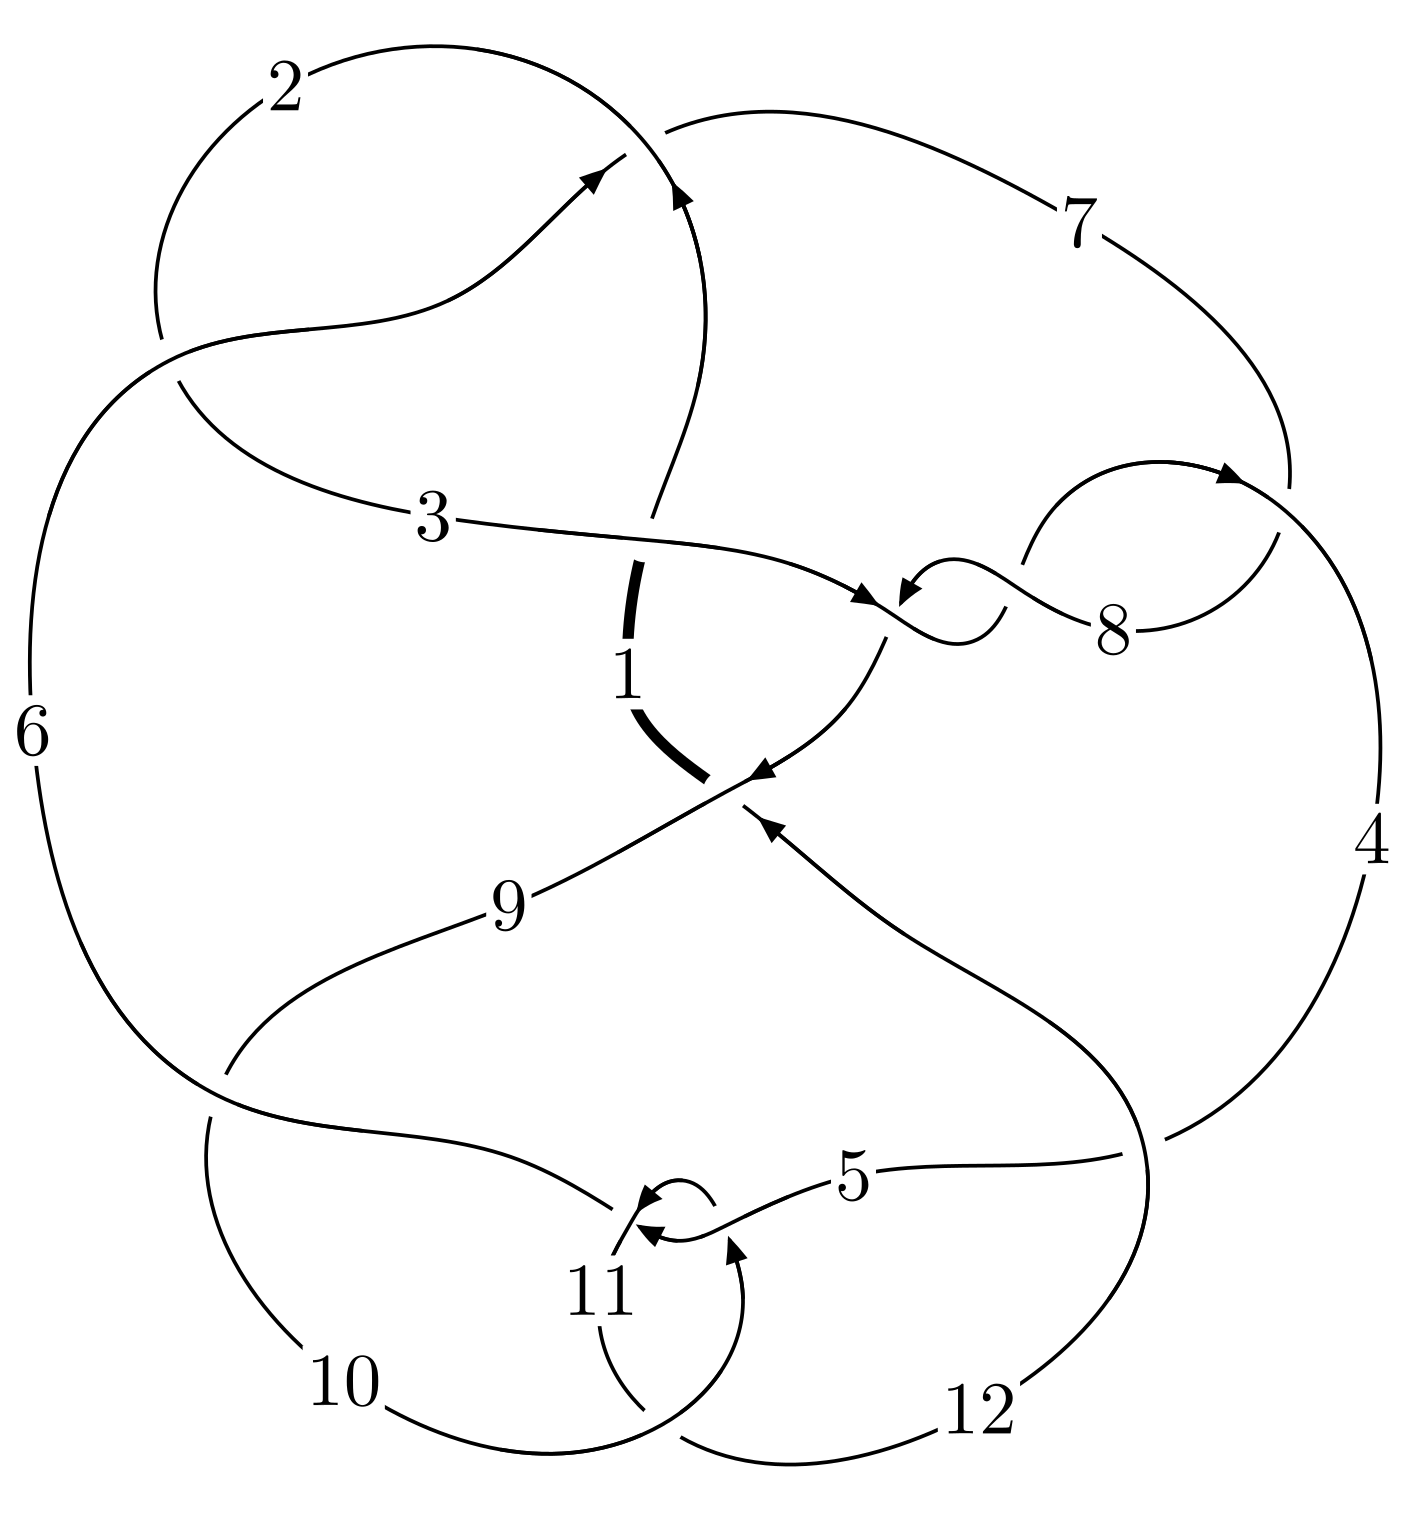
\includegraphics[width=112pt]{../../../GIT/diagram.site/Diagrams/png/2653_12n_0564.png}\\
\ \ \ A knot diagram\footnotemark}&
\allowdisplaybreaks
\textbf{Linearized knot diagam} \\
\cline{2-2}
 &
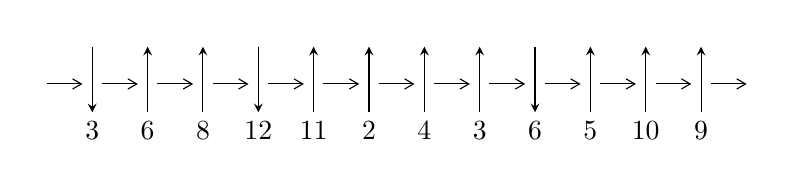
\begin{tikzpicture}[x=20pt, y=17pt]
	% nodes
	\node (C0) at (0, 0) {};
	\node (C1) at (1, 0) {};
	\node (C1U) at (1, +1) {};
	\node (C1D) at (1, -1) {3};

	\node (C2) at (2, 0) {};
	\node (C2U) at (2, +1) {};
	\node (C2D) at (2, -1) {6};

	\node (C3) at (3, 0) {};
	\node (C3U) at (3, +1) {};
	\node (C3D) at (3, -1) {8};

	\node (C4) at (4, 0) {};
	\node (C4U) at (4, +1) {};
	\node (C4D) at (4, -1) {12};

	\node (C5) at (5, 0) {};
	\node (C5U) at (5, +1) {};
	\node (C5D) at (5, -1) {11};

	\node (C6) at (6, 0) {};
	\node (C6U) at (6, +1) {};
	\node (C6D) at (6, -1) {2};

	\node (C7) at (7, 0) {};
	\node (C7U) at (7, +1) {};
	\node (C7D) at (7, -1) {4};

	\node (C8) at (8, 0) {};
	\node (C8U) at (8, +1) {};
	\node (C8D) at (8, -1) {3};

	\node (C9) at (9, 0) {};
	\node (C9U) at (9, +1) {};
	\node (C9D) at (9, -1) {6};

	\node (C10) at (10, 0) {};
	\node (C10U) at (10, +1) {};
	\node (C10D) at (10, -1) {5};

	\node (C11) at (11, 0) {};
	\node (C11U) at (11, +1) {};
	\node (C11D) at (11, -1) {10};

	\node (C12) at (12, 0) {};
	\node (C12U) at (12, +1) {};
	\node (C12D) at (12, -1) {9};
	\node (C13) at (13, 0) {};

	% arrows
	\draw[->,>={angle 60}]
	(C0) edge (C1) (C1) edge (C2) (C2) edge (C3) (C3) edge (C4) (C4) edge (C5) (C5) edge (C6) (C6) edge (C7) (C7) edge (C8) (C8) edge (C9) (C9) edge (C10) (C10) edge (C11) (C11) edge (C12) (C12) edge (C13) ;	\draw[->,>=stealth]
	(C1U) edge (C1D) (C2D) edge (C2U) (C3D) edge (C3U) (C4U) edge (C4D) (C5D) edge (C5U) (C6D) edge (C6U) (C7D) edge (C7U) (C8D) edge (C8U) (C9U) edge (C9D) (C10D) edge (C10U) (C11D) edge (C11U) (C12D) edge (C12U) ;
	\end{tikzpicture} \\
\hhline{~~} \\& 
\textbf{Solving Sequence} \\ \cline{2-2} 
 &
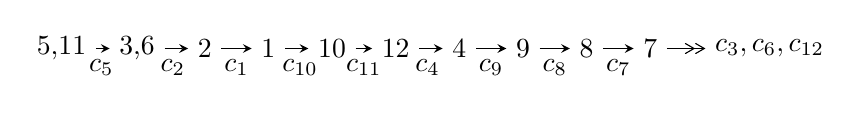
\begin{tikzpicture}[x=23pt, y=7pt]
	% node
	\node (A0) at (-1/8, 0) {5,11};
	\node (A1) at (17/16, 0) {3,6};
	\node (A2) at (17/8, 0) {2};
	\node (A3) at (25/8, 0) {1};
	\node (A4) at (33/8, 0) {10};
	\node (A5) at (41/8, 0) {12};
	\node (A6) at (49/8, 0) {4};
	\node (A7) at (57/8, 0) {9};
	\node (A8) at (65/8, 0) {8};
	\node (A9) at (73/8, 0) {7};
	\node (C1) at (1/2, -1) {$c_{5}$};
	\node (C2) at (13/8, -1) {$c_{2}$};
	\node (C3) at (21/8, -1) {$c_{1}$};
	\node (C4) at (29/8, -1) {$c_{10}$};
	\node (C5) at (37/8, -1) {$c_{11}$};
	\node (C6) at (45/8, -1) {$c_{4}$};
	\node (C7) at (53/8, -1) {$c_{9}$};
	\node (C8) at (61/8, -1) {$c_{8}$};
	\node (C9) at (69/8, -1) {$c_{7}$};
	\node (A10) at (11, 0) {$c_{3},c_{6},c_{12}$};

	% edge
	\draw[->,>=stealth]	
	(A0) edge (A1) (A1) edge (A2) (A2) edge (A3) (A3) edge (A4) (A4) edge (A5) (A5) edge (A6) (A6) edge (A7) (A7) edge (A8) (A8) edge (A9) ;
	\draw[->>,>={angle 60}]	
	(A9) edge (A10);
\end{tikzpicture} \\ 

\end{tabular} \\

\footnotetext{
The image of knot diagram is generated by the software ``\textbf{Draw programme}" developed by Andrew Bartholomew(\url{http://www.layer8.co.uk/maths/draw/index.htm\#Running-draw}), where we modified some parts for our purpose(\url{https://github.com/CATsTAILs/LinksPainter}).
}\phantom \\ \newline 
\centering \textbf{Ideals for irreducible components\footnotemark of $X_{\text{par}}$} 
 
\begin{align*}
I^u_{1}&=\langle 
- u^{16}-3 u^{15}+\cdots+b+3,\;3 u^{16}+7 u^{15}+\cdots+2 a-7,\;u^{17}+3 u^{16}+\cdots-5 u-2\rangle \\
I^u_{2}&=\langle 
u^5 a+u^5-2 u^3 a+u^2 a- u^3+2 a u+b+u+1,\;2 u^4 a+2 u^5- u^3 a- u^4-2 u^2 a-2 u^3+a^2+2 a u+u^2- u,\\
\phantom{I^u_{2}}&\phantom{= \langle  }u^6- u^5- u^4+2 u^3- u+1\rangle \\
I^u_{3}&=\langle 
u^6-2 u^4+u^3+u^2+b- u+1,\;u^8+u^7-3 u^6-2 u^5+3 u^4+u^3+u^2+a+u-2,\;u^{10}-3 u^8+4 u^6- u^4- u^2+1\rangle \\
\\
\end{align*}
\raggedright * 3 irreducible components of $\dim_{\mathbb{C}}=0$, with total 39 representations.\\
\footnotetext{All coefficients of polynomials are rational numbers. But the coefficients are sometimes approximated in decimal forms when there is not enough margin.}
\newpage
\renewcommand{\arraystretch}{1}
\centering \section*{I. $I^u_{1}= \langle - u^{16}-3 u^{15}+\cdots+b+3,\;3 u^{16}+7 u^{15}+\cdots+2 a-7,\;u^{17}+3 u^{16}+\cdots-5 u-2 \rangle$}
\flushleft \textbf{(i) Arc colorings}\\
\begin{tabular}{m{7pt} m{180pt} m{7pt} m{180pt} }
\flushright $a_{5}=$&$\begin{pmatrix}1\\0\end{pmatrix}$ \\
\flushright $a_{11}=$&$\begin{pmatrix}0\\u\end{pmatrix}$ \\
\flushright $a_{3}=$&$\begin{pmatrix}-\frac{3}{2} u^{16}-\frac{7}{2} u^{15}+\cdots+\frac{11}{2} u+\frac{7}{2}\\u^{16}+3 u^{15}+\cdots-5 u-3\end{pmatrix}$ \\
\flushright $a_{6}=$&$\begin{pmatrix}1\\- u^2\end{pmatrix}$ \\
\flushright $a_{2}=$&$\begin{pmatrix}-\frac{5}{2} u^{16}-\frac{11}{2} u^{15}+\cdots+\frac{17}{2} u+\frac{9}{2}\\2 u^{16}+5 u^{15}+\cdots-8 u-5\end{pmatrix}$ \\
\flushright $a_{1}=$&$\begin{pmatrix}u^{11}-2 u^9+2 u^7+u^3\\- u^{13}+3 u^{11}-5 u^9+4 u^7-2 u^5- u^3+u\end{pmatrix}$ \\
\flushright $a_{10}=$&$\begin{pmatrix}- u\\u\end{pmatrix}$ \\
\flushright $a_{12}=$&$\begin{pmatrix}u^3\\- u^3+u\end{pmatrix}$ \\
\flushright $a_{4}=$&$\begin{pmatrix}u^6- u^4+1\\- u^6+2 u^4- u^2\end{pmatrix}$ \\
\flushright $a_{9}=$&$\begin{pmatrix}- u^3\\u^5- u^3+u\end{pmatrix}$ \\
\flushright $a_{8}=$&$\begin{pmatrix}\frac{1}{2} u^{16}+\frac{3}{2} u^{15}+\cdots-\frac{5}{2} u-\frac{3}{2}\\u^{16}+2 u^{15}+\cdots-2 u-1\end{pmatrix}$ \\
\flushright $a_{7}=$&$\begin{pmatrix}-\frac{1}{2} u^{16}-\frac{1}{2} u^{15}+\cdots+\frac{1}{2} u-\frac{1}{2}\\u^{16}+2 u^{15}+\cdots-2 u-1\end{pmatrix}$\\&\end{tabular}
\flushleft \textbf{(ii) Obstruction class $= -1$}\\~\\
\flushleft \textbf{(iii) Cusp Shapes $= -2 u^{16}-4 u^{15}+6 u^{14}+22 u^{13}+2 u^{12}-44 u^{11}-38 u^{10}+30 u^9+64 u^8+26 u^7-36 u^6-48 u^5-16 u^4+18 u^3+12 u^2+8 u+6$}\\~\\
\newpage\renewcommand{\arraystretch}{1}
\flushleft \textbf{(iv) u-Polynomials at the component}\newline \\
\begin{tabular}{m{50pt}|m{274pt}}
Crossings & \hspace{64pt}u-Polynomials at each crossing \\
\hline $$\begin{aligned}c_{1}\end{aligned}$$&$\begin{aligned}
&u^{17}+30 u^{16}+\cdots-8 u-1
\end{aligned}$\\
\hline $$\begin{aligned}c_{2},c_{3},c_{6}\\c_{7},c_{8}\end{aligned}$$&$\begin{aligned}
&u^{17}+15 u^{15}+\cdots+2 u-1
\end{aligned}$\\
\hline $$\begin{aligned}c_{4},c_{9}\end{aligned}$$&$\begin{aligned}
&u^{17}+9 u^{16}+\cdots-77 u-26
\end{aligned}$\\
\hline $$\begin{aligned}c_{5},c_{10}\end{aligned}$$&$\begin{aligned}
&u^{17}+3 u^{16}+\cdots-5 u-2
\end{aligned}$\\
\hline $$\begin{aligned}c_{11}\end{aligned}$$&$\begin{aligned}
&u^{17}-9 u^{16}+\cdots+5 u-4
\end{aligned}$\\
\hline $$\begin{aligned}c_{12}\end{aligned}$$&$\begin{aligned}
&u^{17}+u^{16}+\cdots+953 u-416
\end{aligned}$\\
\hline
\end{tabular}\\~\\
\newpage\renewcommand{\arraystretch}{1}
\flushleft \textbf{(v) Riley Polynomials at the component}\newline \\
\begin{tabular}{m{50pt}|m{274pt}}
Crossings & \hspace{64pt}Riley Polynomials at each crossing \\
\hline $$\begin{aligned}c_{1}\end{aligned}$$&$\begin{aligned}
&y^{17}-98 y^{16}+\cdots+64 y-1
\end{aligned}$\\
\hline $$\begin{aligned}c_{2},c_{3},c_{6}\\c_{7},c_{8}\end{aligned}$$&$\begin{aligned}
&y^{17}+30 y^{16}+\cdots-8 y-1
\end{aligned}$\\
\hline $$\begin{aligned}c_{4},c_{9}\end{aligned}$$&$\begin{aligned}
&y^{17}+11 y^{16}+\cdots+3589 y-676
\end{aligned}$\\
\hline $$\begin{aligned}c_{5},c_{10}\end{aligned}$$&$\begin{aligned}
&y^{17}-9 y^{16}+\cdots+5 y-4
\end{aligned}$\\
\hline $$\begin{aligned}c_{11}\end{aligned}$$&$\begin{aligned}
&y^{17}- y^{16}+\cdots+193 y-16
\end{aligned}$\\
\hline $$\begin{aligned}c_{12}\end{aligned}$$&$\begin{aligned}
&y^{17}+83 y^{16}+\cdots+3035633 y-173056
\end{aligned}$\\
\hline
\end{tabular}\\~\\
\newpage\flushleft \textbf{(vi) Complex Volumes and Cusp Shapes}
$$\begin{array}{c|c|c}  
\text{Solutions to }I^u_{1}& \I (\text{vol} + \sqrt{-1}CS) & \text{Cusp shape}\\
 \hline 
\begin{aligned}
u &= -0.270803 + 0.900641 I \\
a &= -0.709209 - 0.184245 I \\
b &= -0.73238 - 2.39254 I\end{aligned}
 & -15.8747 + 5.8792 I & \phantom{-}1.30073 - 1.97139 I \\ \hline\begin{aligned}
u &= -0.270803 - 0.900641 I \\
a &= -0.709209 + 0.184245 I \\
b &= -0.73238 + 2.39254 I\end{aligned}
 & -15.8747 - 5.8792 I & \phantom{-}1.30073 + 1.97139 I \\ \hline\begin{aligned}
u &= -0.810610 + 0.750728 I \\
a &= -1.317050 + 0.001505 I \\
b &= \phantom{-}0.058875 + 0.461436 I\end{aligned}
 & -19.2384 - 2.7966 I & \phantom{-}0.86008 + 2.64584 I \\ \hline\begin{aligned}
u &= -0.810610 - 0.750728 I \\
a &= -1.317050 - 0.001505 I \\
b &= \phantom{-}0.058875 - 0.461436 I\end{aligned}
 & -19.2384 + 2.7966 I & \phantom{-}0.86008 - 2.64584 I \\ \hline\begin{aligned}
u &= -0.776721 + 0.418654 I \\
a &= \phantom{-}0.541225 + 0.547668 I \\
b &= -0.518708 - 0.343588 I\end{aligned}
 & -0.92435 - 1.82362 I & \phantom{-}3.05958 + 5.69158 I \\ \hline\begin{aligned}
u &= -0.776721 - 0.418654 I \\
a &= \phantom{-}0.541225 - 0.547668 I \\
b &= -0.518708 + 0.343588 I\end{aligned}
 & -0.92435 + 1.82362 I & \phantom{-}3.05958 - 5.69158 I \\ \hline\begin{aligned}
u &= \phantom{-}1.158560 + 0.445647 I \\
a &= -0.511951 + 0.740081 I \\
b &= \phantom{-}0.883342 + 0.177811 I\end{aligned}
 & \phantom{-}4.23482 + 2.69674 I & \phantom{-}10.58660 + 0.80633 I \\ \hline\begin{aligned}
u &= \phantom{-}1.158560 - 0.445647 I \\
a &= -0.511951 - 0.740081 I \\
b &= \phantom{-}0.883342 - 0.177811 I\end{aligned}
 & \phantom{-}4.23482 - 2.69674 I & \phantom{-}10.58660 - 0.80633 I \\ \hline\begin{aligned}
u &= -1.172560 + 0.461545 I \\
a &= -1.225960 + 0.029576 I \\
b &= \phantom{-}1.068970 - 0.795251 I\end{aligned}
 & \phantom{-}4.11934 - 5.61810 I & \phantom{-}10.07697 + 8.39649 I \\ \hline\begin{aligned}
u &= -1.172560 - 0.461545 I \\
a &= -1.225960 - 0.029576 I \\
b &= \phantom{-}1.068970 + 0.795251 I\end{aligned}
 & \phantom{-}4.11934 + 5.61810 I & \phantom{-}10.07697 - 8.39649 I\\
 \hline 
 \end{array}$$\newpage$$\begin{array}{c|c|c}  
\text{Solutions to }I^u_{1}& \I (\text{vol} + \sqrt{-1}CS) & \text{Cusp shape}\\
 \hline 
\begin{aligned}
u &= \phantom{-}1.277260 + 0.264559 I \\
a &= \phantom{-}0.07926 - 2.43683 I \\
b &= -1.56412 + 1.91811 I\end{aligned}
 & -10.78020 - 2.11031 I & \phantom{-}5.71043 + 0.08866 I \\ \hline\begin{aligned}
u &= \phantom{-}1.277260 - 0.264559 I \\
a &= \phantom{-}0.07926 + 2.43683 I \\
b &= -1.56412 - 1.91811 I\end{aligned}
 & -10.78020 + 2.11031 I & \phantom{-}5.71043 - 0.08866 I \\ \hline\begin{aligned}
u &= -0.050223 + 0.684600 I \\
a &= \phantom{-}0.511482 - 0.219170 I \\
b &= \phantom{-}0.581679 + 0.400436 I\end{aligned}
 & \phantom{-}0.95257 + 1.33285 I & \phantom{-}6.82195 - 5.20077 I \\ \hline\begin{aligned}
u &= -0.050223 - 0.684600 I \\
a &= \phantom{-}0.511482 + 0.219170 I \\
b &= \phantom{-}0.581679 - 0.400436 I\end{aligned}
 & \phantom{-}0.95257 - 1.33285 I & \phantom{-}6.82195 + 5.20077 I \\ \hline\begin{aligned}
u &= \phantom{-}0.682195\phantom{ +0.000000I} \\
a &= \phantom{-}0.679402\phantom{ +0.000000I} \\
b &= \phantom{-}0.0468590\phantom{ +0.000000I}\end{aligned}
 & \phantom{-}0.845049\phantom{ +0.000000I} & \phantom{-}13.0200\phantom{ +0.000000I} \\ \hline\begin{aligned}
u &= -1.196000 + 0.589565 I \\
a &= \phantom{-}2.54251 - 1.12472 I \\
b &= -0.80109 + 2.93271 I\end{aligned}
 & -13.0820 - 11.3274 I & \phantom{-}4.07376 + 5.51607 I \\ \hline\begin{aligned}
u &= -1.196000 - 0.589565 I \\
a &= \phantom{-}2.54251 + 1.12472 I \\
b &= -0.80109 - 2.93271 I\end{aligned}
 & -13.0820 + 11.3274 I & \phantom{-}4.07376 - 5.51607 I\\
 \hline 
 \end{array}$$\newpage\newpage\renewcommand{\arraystretch}{1}
\centering \section*{II. $I^u_{2}= \langle u^5 a+u^5-2 u^3 a+u^2 a- u^3+2 a u+b+u+1,\;2 u^4 a+2 u^5+\cdots+a^2- u,\;u^6- u^5- u^4+2 u^3- u+1 \rangle$}
\flushleft \textbf{(i) Arc colorings}\\
\begin{tabular}{m{7pt} m{180pt} m{7pt} m{180pt} }
\flushright $a_{5}=$&$\begin{pmatrix}1\\0\end{pmatrix}$ \\
\flushright $a_{11}=$&$\begin{pmatrix}0\\u\end{pmatrix}$ \\
\flushright $a_{3}=$&$\begin{pmatrix}a\\- u^5 a- u^5+2 u^3 a- u^2 a+u^3-2 a u- u-1\end{pmatrix}$ \\
\flushright $a_{6}=$&$\begin{pmatrix}1\\- u^2\end{pmatrix}$ \\
\flushright $a_{2}=$&$\begin{pmatrix}u^5 a+u^5-2 u^3 a- u^3+2 a u+a+u+1\\- u^5 a+u^4 a-2 u^5+2 u^3 a+u^4-2 u^2 a+2 u^3-2 a u-2 u^2+a- u\end{pmatrix}$ \\
\flushright $a_{1}=$&$\begin{pmatrix}2 u^3+1\\-2 u^3+2 u\end{pmatrix}$ \\
\flushright $a_{10}=$&$\begin{pmatrix}- u\\u\end{pmatrix}$ \\
\flushright $a_{12}=$&$\begin{pmatrix}u^3\\- u^3+u\end{pmatrix}$ \\
\flushright $a_{4}=$&$\begin{pmatrix}u^5-2 u^3+u\\- u^5+u^4+2 u^3- u^2- u+1\end{pmatrix}$ \\
\flushright $a_{9}=$&$\begin{pmatrix}- u^3\\u^5- u^3+u\end{pmatrix}$ \\
\flushright $a_{8}=$&$\begin{pmatrix}u^5 a- u^3 a+2 u^4- u^3+a u-2 u^2+a+2 u+1\\- u^5 a+u^4 a- u^5+u^3 a-2 u^2 a+2 u^3- u^2+a-2 u+1\end{pmatrix}$ \\
\flushright $a_{7}=$&$\begin{pmatrix}- u^5 a- u^5+2 u^3 a+2 u^4- u^2 a+u^3-2 a u-2 u^2+a+u+1\\u^5 a-2 u^3 a- u^4+u^2 a+2 a u- a- u\end{pmatrix}$\\&\end{tabular}
\flushleft \textbf{(ii) Obstruction class $= -1$}\\~\\
\flushleft \textbf{(iii) Cusp Shapes $= -4 u^4+4 u^2-4 u+2$}\\~\\
\newpage\renewcommand{\arraystretch}{1}
\flushleft \textbf{(iv) u-Polynomials at the component}\newline \\
\begin{tabular}{m{50pt}|m{274pt}}
Crossings & \hspace{64pt}u-Polynomials at each crossing \\
\hline $$\begin{aligned}c_{1}\end{aligned}$$&$\begin{aligned}
&u^{12}+15 u^{11}+\cdots+1324 u+289
\end{aligned}$\\
\hline $$\begin{aligned}c_{2},c_{3},c_{6}\\c_{7},c_{8}\end{aligned}$$&$\begin{aligned}
&u^{12}- u^{11}+\cdots-28 u+17
\end{aligned}$\\
\hline $$\begin{aligned}c_{4},c_{9},c_{11}\end{aligned}$$&$\begin{aligned}
&(u^6-3 u^5+5 u^4-4 u^3+2 u^2- u+1)^2
\end{aligned}$\\
\hline $$\begin{aligned}c_{5},c_{10},c_{12}\end{aligned}$$&$\begin{aligned}
&(u^6- u^5- u^4+2 u^3- u+1)^2
\end{aligned}$\\
\hline
\end{tabular}\\~\\
\newpage\renewcommand{\arraystretch}{1}
\flushleft \textbf{(v) Riley Polynomials at the component}\newline \\
\begin{tabular}{m{50pt}|m{274pt}}
Crossings & \hspace{64pt}Riley Polynomials at each crossing \\
\hline $$\begin{aligned}c_{1}\end{aligned}$$&$\begin{aligned}
&y^{12}-13 y^{11}+\cdots+423772 y+83521
\end{aligned}$\\
\hline $$\begin{aligned}c_{2},c_{3},c_{6}\\c_{7},c_{8}\end{aligned}$$&$\begin{aligned}
&y^{12}+15 y^{11}+\cdots+1324 y+289
\end{aligned}$\\
\hline $$\begin{aligned}c_{4},c_{9},c_{11}\end{aligned}$$&$\begin{aligned}
&(y^6+y^5+5 y^4+6 y^2+3 y+1)^2
\end{aligned}$\\
\hline $$\begin{aligned}c_{5},c_{10},c_{12}\end{aligned}$$&$\begin{aligned}
&(y^6-3 y^5+5 y^4-4 y^3+2 y^2- y+1)^2
\end{aligned}$\\
\hline
\end{tabular}\\~\\
\newpage\flushleft \textbf{(vi) Complex Volumes and Cusp Shapes}
$$\begin{array}{c|c|c}  
\text{Solutions to }I^u_{2}& \I (\text{vol} + \sqrt{-1}CS) & \text{Cusp shape}\\
 \hline 
\begin{aligned}
u &= -1.002190 + 0.295542 I \\
a &= \phantom{-}0.912198 - 0.739675 I \\
b &= -0.414477 - 0.040596 I\end{aligned}
 & -1.39926 - 0.92430 I & \phantom{-}7.71672 + 0.79423 I \\ \hline\begin{aligned}
u &= -1.002190 + 0.295542 I \\
a &= \phantom{-}1.20218 + 2.00149 I \\
b &= -1.84373 - 0.52857 I\end{aligned}
 & -1.39926 - 0.92430 I & \phantom{-}7.71672 + 0.79423 I \\ \hline\begin{aligned}
u &= -1.002190 - 0.295542 I \\
a &= \phantom{-}0.912198 + 0.739675 I \\
b &= -0.414477 + 0.040596 I\end{aligned}
 & -1.39926 + 0.92430 I & \phantom{-}7.71672 - 0.79423 I \\ \hline\begin{aligned}
u &= -1.002190 - 0.295542 I \\
a &= \phantom{-}1.20218 - 2.00149 I \\
b &= -1.84373 + 0.52857 I\end{aligned}
 & -1.39926 + 0.92430 I & \phantom{-}7.71672 - 0.79423 I \\ \hline\begin{aligned}
u &= \phantom{-}0.428243 + 0.664531 I \\
a &= -0.486207 + 0.830594 I \\
b &= \phantom{-}0.015656 - 0.966738 I\end{aligned}
 & -5.18047 - 0.92430 I & \phantom{-}0.283283 + 0.794226 I \\ \hline\begin{aligned}
u &= \phantom{-}0.428243 + 0.664531 I \\
a &= -0.860954 - 0.361329 I \\
b &= -1.09861 + 1.55912 I\end{aligned}
 & -5.18047 - 0.92430 I & \phantom{-}0.283283 + 0.794226 I \\ \hline\begin{aligned}
u &= \phantom{-}0.428243 - 0.664531 I \\
a &= -0.486207 - 0.830594 I \\
b &= \phantom{-}0.015656 + 0.966738 I\end{aligned}
 & -5.18047 + 0.92430 I & \phantom{-}0.283283 - 0.794226 I \\ \hline\begin{aligned}
u &= \phantom{-}0.428243 - 0.664531 I \\
a &= -0.860954 + 0.361329 I \\
b &= -1.09861 - 1.55912 I\end{aligned}
 & -5.18047 + 0.92430 I & \phantom{-}0.283283 - 0.794226 I \\ \hline\begin{aligned}
u &= \phantom{-}1.073950 + 0.558752 I \\
a &= -1.37466 - 0.68992 I \\
b &= \phantom{-}0.524769 + 0.629076 I\end{aligned}
 & -3.28987 + 5.69302 I & \phantom{-}4.00000 - 5.51057 I \\ \hline\begin{aligned}
u &= \phantom{-}1.073950 + 0.558752 I \\
a &= \phantom{-}2.60745 - 0.30647 I \\
b &= -1.68361 - 1.82922 I\end{aligned}
 & -3.28987 + 5.69302 I & \phantom{-}4.00000 - 5.51057 I\\
 \hline 
 \end{array}$$\newpage$$\begin{array}{c|c|c}  
\text{Solutions to }I^u_{2}& \I (\text{vol} + \sqrt{-1}CS) & \text{Cusp shape}\\
 \hline 
\begin{aligned}
u &= \phantom{-}1.073950 - 0.558752 I \\
a &= -1.37466 + 0.68992 I \\
b &= \phantom{-}0.524769 - 0.629076 I\end{aligned}
 & -3.28987 - 5.69302 I & \phantom{-}4.00000 + 5.51057 I \\ \hline\begin{aligned}
u &= \phantom{-}1.073950 - 0.558752 I \\
a &= \phantom{-}2.60745 + 0.30647 I \\
b &= -1.68361 + 1.82922 I\end{aligned}
 & -3.28987 - 5.69302 I & \phantom{-}4.00000 + 5.51057 I\\
 \hline 
 \end{array}$$\newpage\newpage\renewcommand{\arraystretch}{1}
\centering \section*{III. $I^u_{3}= \langle u^6-2 u^4+u^3+u^2+b- u+1,\;u^8+u^7+\cdots+a-2,\;u^{10}-3 u^8+4 u^6- u^4- u^2+1 \rangle$}
\flushleft \textbf{(i) Arc colorings}\\
\begin{tabular}{m{7pt} m{180pt} m{7pt} m{180pt} }
\flushright $a_{5}=$&$\begin{pmatrix}1\\0\end{pmatrix}$ \\
\flushright $a_{11}=$&$\begin{pmatrix}0\\u\end{pmatrix}$ \\
\flushright $a_{3}=$&$\begin{pmatrix}- u^8- u^7+3 u^6+2 u^5-3 u^4- u^3- u^2- u+2\\- u^6+2 u^4- u^3- u^2+u-1\end{pmatrix}$ \\
\flushright $a_{6}=$&$\begin{pmatrix}1\\- u^2\end{pmatrix}$ \\
\flushright $a_{2}=$&$\begin{pmatrix}u^9- u^8-3 u^7+3 u^6+3 u^5-3 u^4+u^3- u^2-2 u+2\\- u^9+3 u^7- u^6-3 u^5+2 u^4- u^3- u^2+2 u-1\end{pmatrix}$ \\
\flushright $a_{1}=$&$\begin{pmatrix}u^9-2 u^7+u^5+2 u^3- u\\- u^9+3 u^7-3 u^5+u\end{pmatrix}$ \\
\flushright $a_{10}=$&$\begin{pmatrix}- u\\u\end{pmatrix}$ \\
\flushright $a_{12}=$&$\begin{pmatrix}u^3\\- u^3+u\end{pmatrix}$ \\
\flushright $a_{4}=$&$\begin{pmatrix}u^6- u^4+1\\- u^6+2 u^4- u^2\end{pmatrix}$ \\
\flushright $a_{9}=$&$\begin{pmatrix}- u^3\\u^5- u^3+u\end{pmatrix}$ \\
\flushright $a_{8}=$&$\begin{pmatrix}- u^8+u^7+2 u^6-2 u^5-2 u^4+u^3- u^2+u+1\\- u^9+u^8+2 u^7-2 u^6- u^5+2 u^4-2 u^3+u\end{pmatrix}$ \\
\flushright $a_{7}=$&$\begin{pmatrix}- u^8+u^7+2 u^6-2 u^5-2 u^4+2 u^3- u^2+u+1\\- u^9+u^8+2 u^7-2 u^6-2 u^5+2 u^4- u^3\end{pmatrix}$\\&\end{tabular}
\flushleft \textbf{(ii) Obstruction class $= 1$}\\~\\
\flushleft \textbf{(iii) Cusp Shapes $= -4 u^8+8 u^6-8 u^4-4 u^2+4$}\\~\\
\newpage\renewcommand{\arraystretch}{1}
\flushleft \textbf{(iv) u-Polynomials at the component}\newline \\
\begin{tabular}{m{50pt}|m{274pt}}
Crossings & \hspace{64pt}u-Polynomials at each crossing \\
\hline $$\begin{aligned}c_{1}\end{aligned}$$&$\begin{aligned}
&(u-1)^{10}
\end{aligned}$\\
\hline $$\begin{aligned}c_{2},c_{3},c_{6}\\c_{7},c_{8}\end{aligned}$$&$\begin{aligned}
&(u^2+1)^5
\end{aligned}$\\
\hline $$\begin{aligned}c_{4},c_{9}\end{aligned}$$&$\begin{aligned}
&u^{10}+5 u^8+8 u^6+3 u^4- u^2+1
\end{aligned}$\\
\hline $$\begin{aligned}c_{5},c_{10}\end{aligned}$$&$\begin{aligned}
&u^{10}-3 u^8+4 u^6- u^4- u^2+1
\end{aligned}$\\
\hline $$\begin{aligned}c_{11}\end{aligned}$$&$\begin{aligned}
&(u^5-3 u^4+4 u^3- u^2- u+1)^2
\end{aligned}$\\
\hline $$\begin{aligned}c_{12}\end{aligned}$$&$\begin{aligned}
&(u^5+u^4-2 u^3- u^2+u-1)^2
\end{aligned}$\\
\hline
\end{tabular}\\~\\
\newpage\renewcommand{\arraystretch}{1}
\flushleft \textbf{(v) Riley Polynomials at the component}\newline \\
\begin{tabular}{m{50pt}|m{274pt}}
Crossings & \hspace{64pt}Riley Polynomials at each crossing \\
\hline $$\begin{aligned}c_{1}\end{aligned}$$&$\begin{aligned}
&(y-1)^{10}
\end{aligned}$\\
\hline $$\begin{aligned}c_{2},c_{3},c_{6}\\c_{7},c_{8}\end{aligned}$$&$\begin{aligned}
&(y+1)^{10}
\end{aligned}$\\
\hline $$\begin{aligned}c_{4},c_{9}\end{aligned}$$&$\begin{aligned}
&(y^5+5 y^4+8 y^3+3 y^2- y+1)^2
\end{aligned}$\\
\hline $$\begin{aligned}c_{5},c_{10}\end{aligned}$$&$\begin{aligned}
&(y^5-3 y^4+4 y^3- y^2- y+1)^2
\end{aligned}$\\
\hline $$\begin{aligned}c_{11}\end{aligned}$$&$\begin{aligned}
&(y^5- y^4+8 y^3-3 y^2+3 y-1)^2
\end{aligned}$\\
\hline $$\begin{aligned}c_{12}\end{aligned}$$&$\begin{aligned}
&(y^5-5 y^4+8 y^3-3 y^2- y-1)^2
\end{aligned}$\\
\hline
\end{tabular}\\~\\
\newpage\flushleft \textbf{(vi) Complex Volumes and Cusp Shapes}
$$\begin{array}{c|c|c}  
\text{Solutions to }I^u_{3}& \I (\text{vol} + \sqrt{-1}CS) & \text{Cusp shape}\\
 \hline 
\begin{aligned}
u &= -0.822375 + 0.339110 I \\
a &= \phantom{-}1.88547 + 1.25135 I \\
b &= -1.75626 - 0.65077 I\end{aligned}
 & -2.96077 - 1.53058 I & \phantom{-}0.51511 + 4.43065 I \\ \hline\begin{aligned}
u &= -0.822375 - 0.339110 I \\
a &= \phantom{-}1.88547 - 1.25135 I \\
b &= -1.75626 + 0.65077 I\end{aligned}
 & -2.96077 + 1.53058 I & \phantom{-}0.51511 - 4.43065 I \\ \hline\begin{aligned}
u &= \phantom{-}0.822375 + 0.339110 I \\
a &= -0.32986 - 1.50891 I \\
b &= -0.656443 + 0.030936 I\end{aligned}
 & -2.96077 + 1.53058 I & \phantom{-}0.51511 - 4.43065 I \\ \hline\begin{aligned}
u &= \phantom{-}0.822375 - 0.339110 I \\
a &= -0.32986 + 1.50891 I \\
b &= -0.656443 - 0.030936 I\end{aligned}
 & -2.96077 - 1.53058 I & \phantom{-}0.51511 + 4.43065 I \\ \hline\begin{aligned}
u &= \phantom{-0.000000 -}0.766826 I \\
a &= \phantom{-}0.821196 + 0.370286 I \\
b &= \phantom{-}0.482881 + 1.217740 I\end{aligned}
 & -0.888787\phantom{ +0.000000I} & \phantom{-}1.48110\phantom{ +0.000000I} \\ \hline\begin{aligned}
u &= \phantom{-0.000000 } -0.766826 I \\
a &= \phantom{-}0.821196 - 0.370286 I \\
b &= \phantom{-}0.482881 - 1.217740 I\end{aligned}
 & -0.888787\phantom{ +0.000000I} & \phantom{-}1.48110\phantom{ +0.000000I} \\ \hline\begin{aligned}
u &= -1.200150 + 0.455697 I \\
a &= -1.56305 + 1.07974 I \\
b &= \phantom{-}0.74575 - 2.04068 I\end{aligned}
 & \phantom{-}2.58269 - 4.40083 I & \phantom{-}4.74431 + 3.49859 I \\ \hline\begin{aligned}
u &= -1.200150 - 0.455697 I \\
a &= -1.56305 - 1.07974 I \\
b &= \phantom{-}0.74575 + 2.04068 I\end{aligned}
 & \phantom{-}2.58269 + 4.40083 I & \phantom{-}4.74431 - 3.49859 I \\ \hline\begin{aligned}
u &= \phantom{-}1.200150 + 0.455697 I \\
a &= \phantom{-}0.186244 + 1.292420 I \\
b &= \phantom{-}1.18408 - 0.79689 I\end{aligned}
 & \phantom{-}2.58269 + 4.40083 I & \phantom{-}4.74431 - 3.49859 I \\ \hline\begin{aligned}
u &= \phantom{-}1.200150 - 0.455697 I \\
a &= \phantom{-}0.186244 - 1.292420 I \\
b &= \phantom{-}1.18408 + 0.79689 I\end{aligned}
 & \phantom{-}2.58269 - 4.40083 I & \phantom{-}4.74431 + 3.49859 I\\
 \hline 
 \end{array}$$\newpage
\newpage\renewcommand{\arraystretch}{1}
\centering \section*{ IV. u-Polynomials}
\begin{tabular}{m{50pt}|m{274pt}}
Crossings & \hspace{64pt}u-Polynomials at each crossing \\
\hline $$\begin{aligned}c_{1}\end{aligned}$$&$\begin{aligned}
&((u-1)^{10})(u^{12}+15 u^{11}+\cdots+1324 u+289)\\
&\cdot(u^{17}+30 u^{16}+\cdots-8 u-1)
\end{aligned}$\\
\hline $$\begin{aligned}c_{2},c_{3},c_{6}\\c_{7},c_{8}\end{aligned}$$&$\begin{aligned}
&((u^2+1)^5)(u^{12}- u^{11}+\cdots-28 u+17)(u^{17}+15 u^{15}+\cdots+2 u-1)
\end{aligned}$\\
\hline $$\begin{aligned}c_{4},c_{9}\end{aligned}$$&$\begin{aligned}
&((u^6-3 u^5+5 u^4-4 u^3+2 u^2- u+1)^{2})(u^{10}+5 u^8+8 u^6+3 u^4- u^2+1)\\
&\cdot(u^{17}+9 u^{16}+\cdots-77 u-26)
\end{aligned}$\\
\hline $$\begin{aligned}c_{5},c_{10}\end{aligned}$$&$\begin{aligned}
&(u^6- u^5- u^4+2 u^3- u+1)^2(u^{10}-3 u^8+4 u^6- u^4- u^2+1)\\
&\cdot(u^{17}+3 u^{16}+\cdots-5 u-2)
\end{aligned}$\\
\hline $$\begin{aligned}c_{11}\end{aligned}$$&$\begin{aligned}
&(u^5-3 u^4+4 u^3- u^2- u+1)^2(u^6-3 u^5+5 u^4-4 u^3+2 u^2- u+1)^2\\
&\cdot(u^{17}-9 u^{16}+\cdots+5 u-4)
\end{aligned}$\\
\hline $$\begin{aligned}c_{12}\end{aligned}$$&$\begin{aligned}
&(u^5+u^4-2 u^3- u^2+u-1)^2(u^6- u^5- u^4+2 u^3- u+1)^2\\
&\cdot(u^{17}+u^{16}+\cdots+953 u-416)
\end{aligned}$\\
\hline
\end{tabular}\newpage\renewcommand{\arraystretch}{1}
\centering \section*{ V. Riley Polynomials}
\begin{tabular}{m{50pt}|m{274pt}}
Crossings & \hspace{64pt}Riley Polynomials at each crossing \\
\hline $$\begin{aligned}c_{1}\end{aligned}$$&$\begin{aligned}
&((y-1)^{10})(y^{12}-13 y^{11}+\cdots+423772 y+83521)\\
&\cdot(y^{17}-98 y^{16}+\cdots+64 y-1)
\end{aligned}$\\
\hline $$\begin{aligned}c_{2},c_{3},c_{6}\\c_{7},c_{8}\end{aligned}$$&$\begin{aligned}
&((y+1)^{10})(y^{12}+15 y^{11}+\cdots+1324 y+289)\\
&\cdot(y^{17}+30 y^{16}+\cdots-8 y-1)
\end{aligned}$\\
\hline $$\begin{aligned}c_{4},c_{9}\end{aligned}$$&$\begin{aligned}
&(y^5+5 y^4+8 y^3+3 y^2- y+1)^2(y^6+y^5+5 y^4+6 y^2+3 y+1)^2\\
&\cdot(y^{17}+11 y^{16}+\cdots+3589 y-676)
\end{aligned}$\\
\hline $$\begin{aligned}c_{5},c_{10}\end{aligned}$$&$\begin{aligned}
&(y^5-3 y^4+4 y^3- y^2- y+1)^2(y^6-3 y^5+5 y^4-4 y^3+2 y^2- y+1)^2\\
&\cdot(y^{17}-9 y^{16}+\cdots+5 y-4)
\end{aligned}$\\
\hline $$\begin{aligned}c_{11}\end{aligned}$$&$\begin{aligned}
&(y^5- y^4+8 y^3-3 y^2+3 y-1)^2(y^6+y^5+5 y^4+6 y^2+3 y+1)^2\\
&\cdot(y^{17}- y^{16}+\cdots+193 y-16)
\end{aligned}$\\
\hline $$\begin{aligned}c_{12}\end{aligned}$$&$\begin{aligned}
&(y^5-5 y^4+8 y^3-3 y^2- y-1)^2(y^6-3 y^5+5 y^4-4 y^3+2 y^2- y+1)^2\\
&\cdot(y^{17}+83 y^{16}+\cdots+3035633 y-173056)
\end{aligned}$\\
\hline
\end{tabular}
\vskip 2pc
\end{document}